\begin{figure}[t]
 \centering
 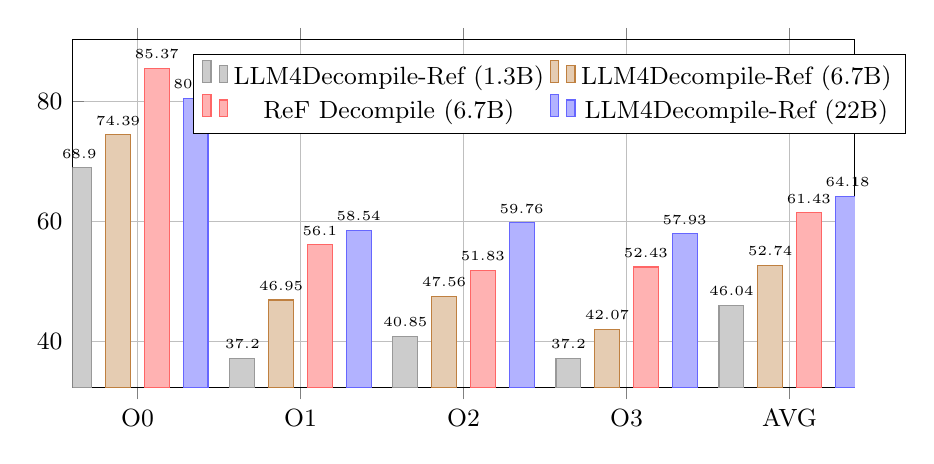
\begin{tikzpicture} 
 \begin{axis}[
 enlargelimits=0.10,
 legend style={at={(0.61,0.96)},
  anchor=north,legend columns=2},
 symbolic x coords={O0, O1, O2, O3, AVG},
 xtick=data,
 ybar=5pt,% configures `bar shift'
 bar width=9pt,
 width=0.95\linewidth, height=6cm,
 nodes near coords,
 nodes near coords align={vertical},
 nodes near coords style={font=\tiny},
 font=\small,
 grid=major,
 ]
 \addplot[fill=black!20!white,draw=black!40!white] coordinates {
  (O0, 68.9)
  (O1, 37.2)
  (O2, 40.85)
  (O3, 37.2)
  (AVG, 46.04)
 };
 \addplot [fill=brown!40!white,draw=brown] coordinates {
  (O0, 74.39)
  (O1, 46.95)
  (O2, 47.56)
  (O3, 42.07)
  (AVG, 52.74)
 };
  \addplot [fill=red!30!white,draw=red!60!white] coordinates {
  (O0, 85.37)
  (O1, 56.1)
  (O2, 51.83)
  (O3, 52.43)
  (AVG, 61.43)
 };
  \addplot [fill=blue!30!white,draw=blue!60!white] coordinates {
  (O0, 80.49)
  (O1, 58.54)
  (O2, 59.76)
  (O3, 57.93)
  (AVG, 64.18)
 };
 \legend{LLM4Decompile-Ref (1.3B), LLM4Decompile-Ref (6.7B), ReF Decompile (6.7B), LLM4Decompile-Ref (22B)}
 \end{axis}
 \end{tikzpicture}
 \caption{Re-executability rate comparison between ReF Decompile and LLM4Decompile-Ref models of varying sizes (1.3B, 6.7B, and 22B parameters).}\label{fig:compare}
\end{figure}